\chapter{相关基础研究}
\label{chapter:background}

本章将介绍普通和加密后重复数据删除、可信计算(TEE)等本文利用的基础知识。

\section{重复数据删除}
\label{sec:background-deduplication}


\begin{figure}[!htb]
    \small
    \centering
    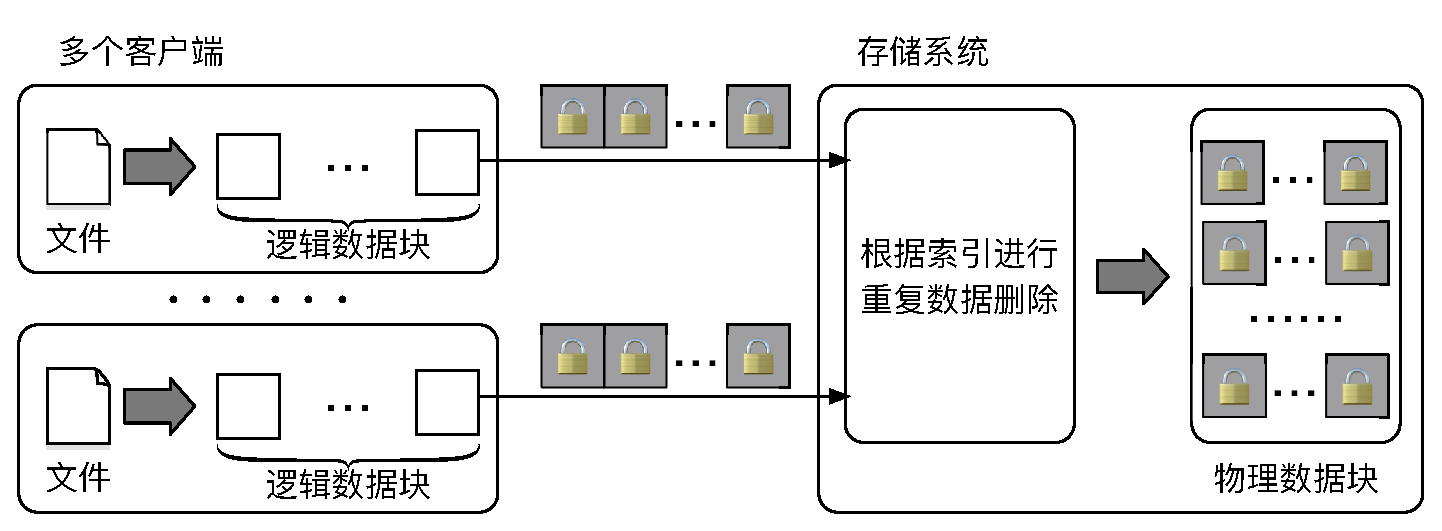
\includegraphics[width=14cm]{DedupSystemView.eps}
    \caption{基于数据块的重复数据删除的工作流程概览} 
    \label{fig:重复数据删除的工作流程概览}
\end{figure}

本文专注于基于数据块的重复数据删除,它以称为数据块的小型数据单元为粒度运行。图\ref{fig:重复数据删除的工作流程概览}总结了重复数据删除工作流程。 

具体地,重复数据删除系统首先通过文件切块过程将客户端的文件(例如,备份文件)分割成逻辑数据块,根据每一个逻辑数据块的内容,使用哈希算法计算得到其对应的唯一标签(又成为指纹)。如果两个数据块具有相同的标签,那么认为两个数据块相同(不同逻辑数据块计算得到相同的标志的概率忽略不计\cite{black2006compare}),即数据块内容和其标志完全一致;若两个逻辑数据块标签不一致,显然两逻辑数据块不同。重复数据删除系统的存储系统仅存储相同逻辑数据块的副本(称为物理数据块),并且每个相同的逻辑数据块通过一个较小空间开销的索引引用相同的物理数据块。  

基于数据块的重复数据删除比基于文件的重复数据删除更精细,因此通常具有更高的存储效率(节省更多的存储空间)。基于数据块的重复数据删除有两种基本的数据块分块方法:固定大小的数据分块方法和可变大小的数据分块方法。固定大小的数据分块方法将数据分割为大小相同的逻辑数据块,而可变大小的数据分块方法(也称为内容定义的数据块分块方法)通常以内容相关的方式指定数据块的边界(例如,通过Rabin指纹识别基于数据块{rabin1981fingerprinting})将文件数据分区为可变大小的数据块。固定大小的分块方法简单而快速,而可变大小的分块方法可以在内容发生变换时保持存储效率,因为即使文件添加或删除了某些内容,大多数数据块仍保持不变。可变大小的分块通常用在备份系统中(例如,\cite{zhu2008avoiding,lillibridge2009sparse}),但固定大小的分块显然对某些工作负载更加有效(例如,VM备份数据集\cite{jin2009effectiveness})。本文的工作同时涉及固定大小和可变大小的分块方法产生的数据块。

加密的重复数据删除解决了外包环境(例如,云存储)中的数据块机密性,同时保持了重复数据删除的有效性。出于安全考虑,用户希望在将自己的数据外包之前对其数据进行加密,以确保个人数据的隐私性。传统的对称加密要求多个客户端通过其(不同的)密钥加密其文件数据,即使相同的明文数据块也会被加密为不同的密文数据块,服务器无法感知到这些密文数据块所对应的的原始明文数据块内容是否相同。消息锁加密(MLE)\cite{bellare2013message}给加密重复数据删除提供了新的处理方法。最基本的MLE实例化是基于每个明文的内容(例如,基于数据块的重复数据删除中的逻辑数据块)导出其对称密钥(称为MLE密钥),并使用MLE密钥加密明文以形成对应的密文数据块(例如,加密的逻辑数据块)。因此,MLE可以确保将相同的明文加密为相同的密文数据块。最后,存储系统从每个密文数据块中导出其对应的标签并执行重复数据删除。

\section{加密重复数据删除(密钥生成技术)}
\label{sec:background-encrypted-deduplication}

\textit{消息锁加密(MLE)} \cite{bellare2013MLE} 将加密原语形式化用于加密后重复数据删除。它指定了对称密钥(称为 \textit{ 消息锁加密(MLE) 密钥})如何从明文数据块的 \textit{ content}(例如,其流行的实例化 \textit{ convergent encryption (CE)} \cite{douceur02}使用明文数据块的加密哈希作为 消息锁加密(MLE) 密钥)。因此,它将重复的明文数据块加密为重复的密文数据块,从而使重复数据删除在密文数据块上仍然可行。

\paragraph*{Server-aided 消息锁加密(MLE).} CE 易受 \textit{ 离线暴力攻击},因为它的 消息锁加密(MLE) 密钥(即明文数据块的哈希)可以公开派生。具体来说,攻击者通过枚举所有可能的明文数据块的 消息锁加密(MLE) 密钥来从目标密文数据块(不知道 消息锁加密(MLE) 密钥)推断输入明文数据块,以检查是否有任何明文数据块被加密到目标密文数据块。

服务器辅助消息锁加密(Server-aided MLE)\cite{bellare2013DupLESS} 是最先进的加密原语,可增强加密后重复数据删除对离线暴力攻击的安全性。

它为消息锁加密(MLE) 中的密钥生成步骤部署了一个专用的 \textit{ 密钥管理器(key server)}。为了加密明文数据块,客户端首先将明文数据块的指纹发送到密钥管理器,密钥管理器通过指纹和密钥管理器维护的\textit{ global secret}返回消息锁加密(MLE) 密钥。如果全局机密是安全的,则对手无法发起离线暴力攻击;否则,如果全局机密被泄露,则安全性会降低到原始 消息锁加密(MLE) 的安全性。服务器辅助 消息锁加密(MLE) 进一步建立在两种安全机制之上。首先,它使用 \textit{ oblivious pseudorandom function (OPRF)} \cite{naor2004Number} 允许客户端发送明文数据块的“盲”指纹,这样密钥管理器仍然可以返回相同的 消息锁加密(MLE) 密钥用于相同指纹无需学习原始指纹。其次,它对来自客户端的密钥生成请求进行速率限制,以防止恶意客户端向密钥管理器发出许多密钥生成请求,以找到目标消息锁加密(MLE) 密钥。

\section{数据所有权证明}
\label{sec:background-pow}

\paragraph*{Proof-of-ownership.} 为了节省带宽,加密后重复数据删除可以应用源端重复数据删除,而不是基于存储目标的重复数据删除,以在客户端删除重复的密文数据块,而无需上传到云(\S\ref{sec:sgxdedup-introduction})。客户端将密文数据块的指纹发送到云端,云端检查指纹是否被指纹索引跟踪(即对应的密文数据块已被存储)。然后,客户端仅将非重复密文数据块上传到云端。


但是,当某些客户端受到威胁时,源端重复数据删除很容易受到 \textit{ side-channel attack} \cite{harnik10,halevi11} 的攻击。一种侧信道攻击是,受感染的客户端可以通过将密文数据块的指纹发送到云来查询任何目标密文数据块的存在(例如,如果密文数据块对应于某个可能的密码 \cite{harnik10}),因此以识别来自其​​他客户端的敏感信息。另一种侧信道攻击是受感染的客户端可以未经授权访问其他客户端的存储块。具体来说,它可以使用任何目标密文数据块的指纹来说服云它是具有完全访问权限 \cite{halevi11} 的相应密文数据块的所有者。


\textit{ 所有权证明 (PoW)} \cite{halevi11} 是一种加密方法,可增强源端重复数据删除,防止侧信道攻击,同时保持源端重复数据删除的带宽节省。

它的想法是让云验证客户端确实是密文数据块的所有者,并被授权完全访问密文数据块。这确保了受感染的客户端无法查询其他客户端的块是否存在。具体来说,在基于 PoW 的源端重复数据删除中,客户端将发送到云的每个指纹都附加一个 \textit{ PoW 证明},云可以通过它验证客户端是否是相应密文数据块的真正所有者。云仅对成功的证明验证做出响应,从而防止任何受感染的客户端识别其他客户端拥有的密文数据块。 

\paragraph*{Limitations.} 回想一下 \S\ref{sec:sgxdedup-introduction},现有的加密后重复数据删除实现需要昂贵的加密保护。服务器辅助 消息锁加密(MLE) 需要 OPRF 协议 \cite{naor2004Number} 来保护指纹信息免受密钥管理器的影响,但 OPRF 协议涉及昂贵的公钥加密操作。例如,本文的评估 (\S\ref{subsec:sgxdedup-synthetic}) 表明,基于 OPRF 的 消息锁加密(MLE) 密钥生成只能达到 25\,MB/s (Exp\#1) 并将整体加密后重复数据删除性能限制在 20 \,MB/s (Exp\#4)。此外,现有的 PoW 实现基于 Merkle-tree 协议 \cite{halevi11},由于块级 PoW 的频繁哈希计算,该协议仅实现 37\,MB/s (Exp\#3)。在 1\,GbE LAN 环境中,PoW 的计算开销甚至抵消了在源端重复数据删除中消除重复数据上传的性能增益。虽然本文可以通过基于每个文件应用 PoW 来减轻 PoW 计算(即,客户端证明其对文件的所有权),但云无法验证块是否属于基于数据块的重复数据删除下的文件。提高服务器辅助 消息锁加密(MLE) 或 PoW 性能的现有解决方案通常会牺牲安全性 \cite{li20b,xu2013weak,pietro12}、带宽效率 \cite{harnik10,li15} 或存储效率 \cite{zhou2015secdep,qin17,li20b} (\S\ref{sec:sgxdedup-related_work})。


\section{可信计算环境(TEE)}
\label{sec:background-tee}


\subsection{Intel SGX}
\label{subsec:background-tee-sgx}

本文探索硬件辅助可信执行以减轻加密后重复数据删除的性能开销,同时保持安全性、带宽效率和存储效率。在这项工作中,本文专注于Intel SGX \cite{sgx},这是一套内置于现代Intel CPU 中的安全相关指令。 SGX 在称为 \textit{ enclave} 的硬件保护环境中屏蔽代码和数据的执行。在下文中,本文将重点介绍与本文的工作相关的安全区的三个安全特性:隔离、证明和密封。

\paragraph*{Isolation.}安全区驻留在称为 \textit{安全区page cache (EPC)} 的硬件保护内存区域中,用于托管任何受保护的代码和数据。一个 EPC 包含 4KB 页面,任何 in-enclave 应用程序最多可占用 96\,MB \cite{harnik18}。如果安全区的大小比 EPC 大,它会加密未使用的页面并将它们驱逐到未受保护的内存中。在这项工作中,本文在每个客户端和密钥管理器中部署安全区以保护敏感操作 (\S\ref{subsec:sgxdedup-arch})。本文还限制了 in-enclave 内容的大小以减轻分页开销 (\S\ref{subsec:sgxdedup-encryption})。

enclave 提供了一个接口,即 \textit{安全区call (ECall)},以便外部应用程序可以发出 ECall 以安全地访问安全区内的内容。请注意,ECall 会产生访问安全区内存 \cite{harnik18} 的上下文切换开销。本文通过批量处理内容来减少 ECall 的数量(\S\ref{sec:sgxdedup-implementation})。

\paragraph*{Attestation.} SGX 支持 \textit{ 远程认证} 通过远程实体(例如云)对目标安全区进行身份验证。在远程证明过程中(详见\cite{sgx}),远程实体需要联系Intel运营的证明服务来检查目标enclave提供的enclave信息的完整性。然后,远程实体通过将其安全区信息与目标安全区中预期的可信配置进行比较来验证目标 enclave。本文使用远程证明来确保在第一个引导程序中将正确的代码和数据加载到每个安全区中。

\paragraph*{Sealing.} SGX 通过密封将安全区内容存储在安全区外部时对其进行保护。它使用秘密 \textit{ 密封密钥} 在被驱逐之前加密数据。密封密钥可以从 \textit{ 测量散列}(即安全区内容的 SHA256 散列)或安全区的作者身份派生,因此只有相应的安全区才能访问密封密钥并解密密封数据.由于远程证明会导致显着延迟(Exp\#7),本文使用密封来消除安全区第一次引导后的远程证明(\S\ref{subsec:sgxdedup-enclave-management})。

\paragraph*{Remarks.} 本文不考虑基于内存加密的 TEE(例如 AMD SEV \cite{AMDSEV} 和 MK-TME \cite{Mktem}),因为它们需要大型可信计算基础并暴露出广泛的攻击面\cite{mofrad18}。此外,AMD SEV \cite{AMDSEV} 不保护内存完整性,并且容易受到特权对手可以操纵加密内存页 \cite{mofrad18} 的攻击。


\subsection{ARM TrustZone}
\label{subsec:background-tee-tz}
